% -*- latex -*-
%%%%%%%%%%%%%%%%%%%%%%%%%%%%%%%%%%%%%%%%%%%%%%%%%%%%%%%%%%%%%%%%
%%%%%%%%%%%%%%%%%%%%%%%%%%%%%%%%%%%%%%%%%%%%%%%%%%%%%%%%%%%%%%%%
%%%%
%%%% This text file is part of the source of 
%%%% `Parallel Computing'
%%%% by Victor Eijkhout, copyright 2012-6
%%%%
%%%% mpiref.tex : MPI reference
%%%%
%%%%%%%%%%%%%%%%%%%%%%%%%%%%%%%%%%%%%%%%%%%%%%%%%%%%%%%%%%%%%%%%
%%%%%%%%%%%%%%%%%%%%%%%%%%%%%%%%%%%%%%%%%%%%%%%%%%%%%%%%%%%%%%%%

This section gives reference information and illustrative examples
of the use of MPI. While the code snippets given here should be enough,
full programs can be found in the repository for this book
\url{https://bitbucket.org/VictorEijkhout/parallel-computing-book}.

\Level 0 {One-sided communication}
\commandreflabel{one-sided}

\Level 1 {Remote memory access}
\commandreflabel{putget}

The \n{MPI_Put} routine is used to put data in the window
of a target process
%
\mpiRoutineRef{MPI_Put}
%
The data is written in the buffer of the target window,
using the window parameters that were specified on the target.
Specifically, data is written starting at
\[ \mathtt{window\_base} + \mathtt{target\_disp}\times \mathtt{disp\_unit}. \]

The \indexmpishow{MPI_Get} call is very similar.
\begin{verbatim}
int MPI_Get(void *origin_addr, int origin_count, MPI_Datatype
            origin_datatype, int target_rank, MPI_Aint target_disp,
            int target_count, MPI_Datatype target_datatype, MPI_Win
            win)
\end{verbatim}

Here is a single put operation. Note that the window create and window fence calls
are collective, so they have to be performed on all processors
of the communicator that was used in the create call.
\verbatimsnippet{putblock}

Very similar, a get operation.
\verbatimsnippet{getblock}

A third one-sided routine
is \n{MPI_Accumulate} which does a reduction operation on the results
that are being put:\indexmpi{MPI_Accumulate}
\begin{verbatim}
MPI_Accumulate (
  void *origin_addr, int origin_count, MPI_Datatype origin_datatype, 
  int target_rank,
  MPI_Aint target_disp, int target_count, MPI_Datatype target_datatype,
  MPI_Op op,MPI_Win window)
\end{verbatim}

\Level 2 {Request-based operations}

Analogous to \n{MPI_Isend} there are request based one-sided operations:
%
\mpiRoutineRef{MPI_Rput}
%
and similarly \indexmpishow{MPI_Rget} and \indexmpishow{MPI_Raccumulate}.

These only apply to passive target synchronization.
Any \indexmpishow{MPI_Win_flush...} call also terminates these transfers.

\Level 1 {Active target synchronization}
\commandreflabel{fence}

\indexmpi{MPI_Win_fence}
\begin{verbatim}
MPI_Win_fence (int assert, MPI_Win win)
\end{verbatim}

\Level 1 {Assertions}
\label{sec:mpi-assert}

The \n{MPI_Win_fence} call, as well \n{MPI_Win_start} and such, take an argument
through which assertions can be passed about the activity before, after, and during the epoch.
The value zero is always allowed, by you can make your program more efficient by specifying
one or more of the following, combined by bitwise OR in C/C++ or
\n{IOR} in Fortran.

\begin{description}
\item[\texttt{MPI\_WIN\_START}] Supports the option:
  \begin{description}
    \item[\texttt{MPI\_MODE\_NOCHECK}] the matching calls to \n{MPI_WIN_POST} have already
    completed on all target processes when the call to \n{MPI_WIN_START} is
    made. The nocheck option can be specified in a start call if and
    only if it is specified in each matching post call. This is similar
    to the optimization of ``ready-send'' that may save a handshake when
    the handshake is implicit in the code. (However, ready-send is
    matched by a regular receive, whereas both start and post must
    specify the nocheck option.)
  \end{description}
\item[\texttt{MPI\_WIN\_POST}] supports the following options:
  \begin{description}
  \item[\texttt{MPI\_MODE\_NOCHECK}] the matching calls to \n{MPI_WIN_START} have not
    yet occurred on any origin processes when the call to \n{MPI_WIN_POST}
    is made. The nocheck option can be specified by a post call if and
    only if it is specified by each matching start call.
  \item[\texttt{MPI\_MODE\_NOSTORE}] the local window was not updated by local
    stores (or local get or receive calls) since last
    synchronization. This may avoid the need for cache synchronization
    at the post call.
  \item[\texttt{MPI\_MODE\_NOPUT}] the local window will not be updated by put or
    accumulate calls after the post call, until the ensuing (wait)
    synchronization. This may avoid the need for cache synchronization
    at the wait call.
  \end{description}
\item[\texttt{MPI\_WIN\_FENCE}] supports the following options:
  \begin{description}
  \item[\texttt{MPI\_MODE\_NOSTORE}] the local window was not updated by local
    stores (or local get or receive calls) since last synchronization.
  \item[\texttt{MPI\_MODE\_NOPUT}] the local window will not be updated by put or
    accumulate calls after the fence call, until the ensuing (fence)
    synchronization.
  \item[\texttt{MPI\_MODE\_NOPRECEDE}] the fence does not complete any sequence of
    locally issued RMA calls. If this assertion is given by any
    process in the window group, then it must be given by all
    processes in the group.
  \item[\texttt{MPI\_MODE\_NOSUCCEED}] the fence does not start any
    sequence of locally issued RMA calls. If the assertion is given by
    any process in the window group, then it must be given by all
    processes in the group.
  \end{description}
\item[\texttt{MPI\_WIN\_LOCK}] supports the following option:
  \begin{description}
    \item[\texttt{MPI\_MODE\_NOCHECK}] no other process holds, or will attempt to
    acquire a conflicting lock, while the caller holds the window
    lock. This is useful when mutual exclusion is achieved by other
    means, but the coherence operations that may be attached to the
    lock and unlock calls are still required.
  \end{description}
\end{description}

\begin{wrapfigure}{r}{3in}
  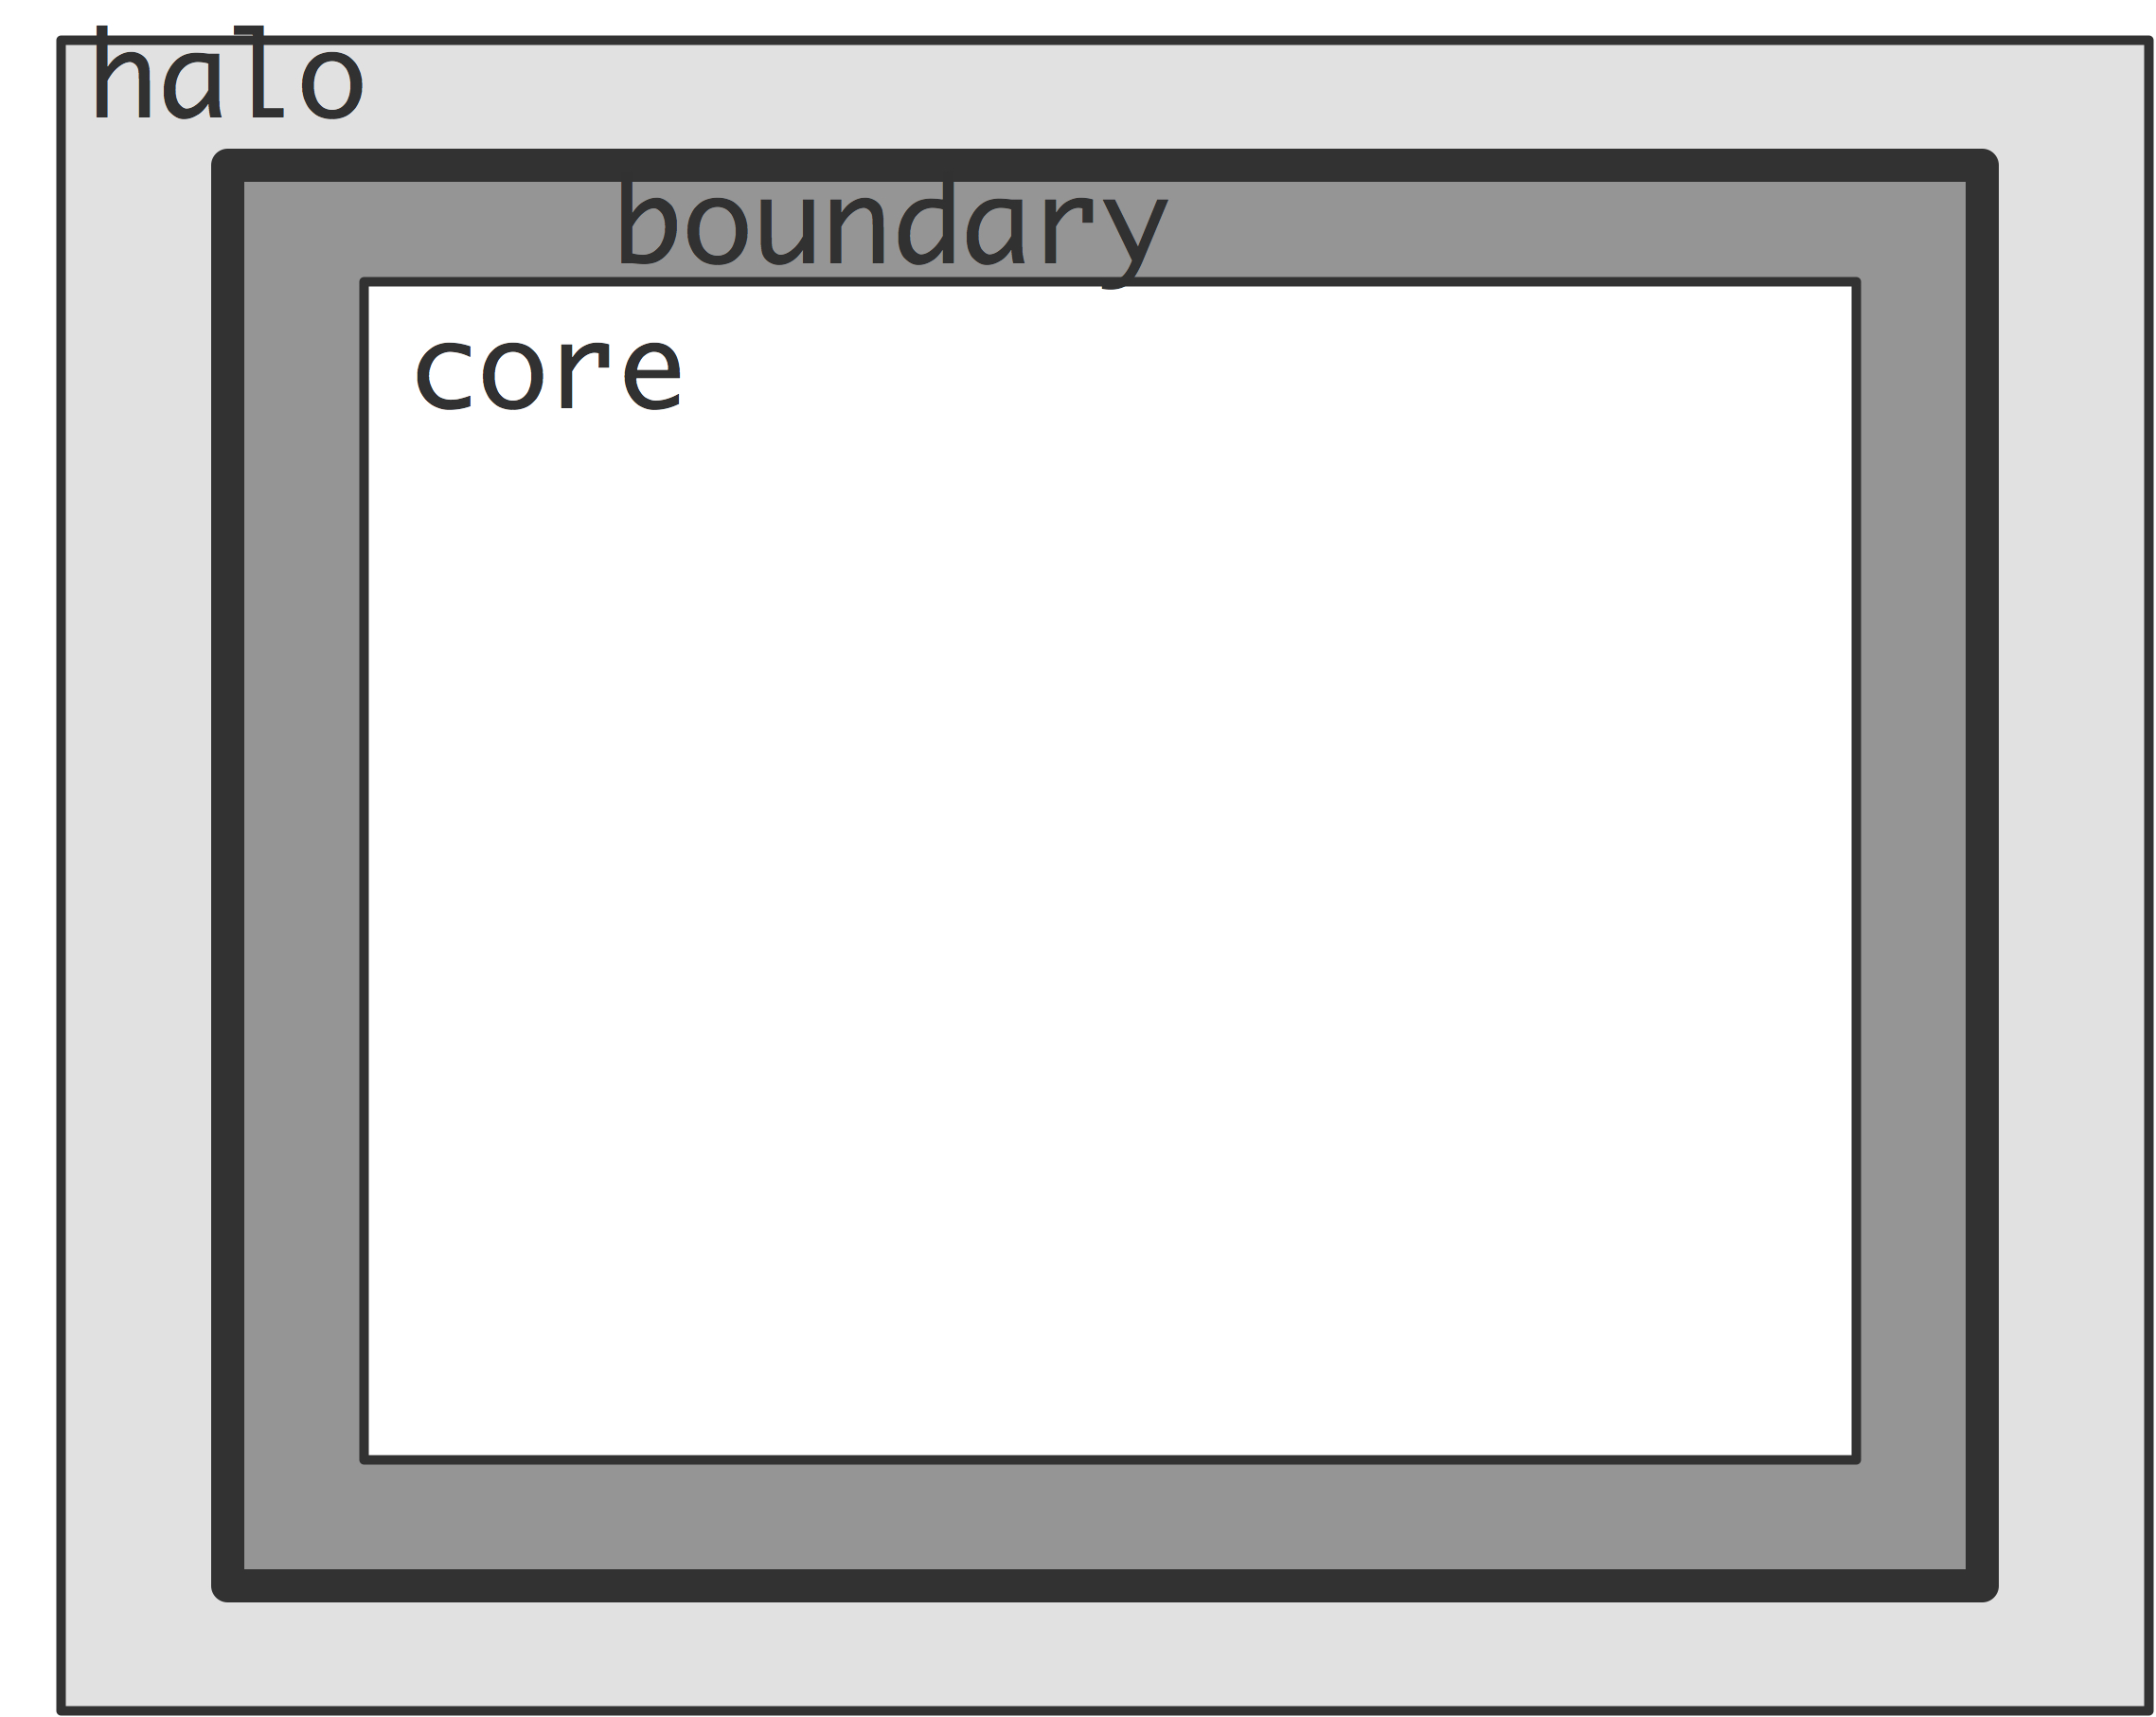
\includegraphics[scale=.08]{core-update}
\end{wrapfigure}
%
As an example, let's look at \indextermbus{halo}{update}.
The array~\n{A} is updated using the local values and the halo
that comes from bordering processors, either through Put or Get operations.

In a first version we separate computation and communication.
Each iteration has two fences. Between the two fences in the loop body
we do the \n{MPI_Put} operation; between the second and and first one
of the next iteration there is only computation, so we add the
\n{NOPRECEDE} and \n{NOSUCCEED} assertions. The \n{NOSTORE} assertion
states that the local window was not updated: the Put operation only
works on remote windows.
\begin{verbatim}
for ( .... ) {
  update(A); 
  MPI_Win_fence(MPI_MODE_NOPRECEDE, win); 
  for(i=0; i < toneighbors; i++) 
    MPI_Put( ... );
  MPI_Win_fence((MPI_MODE_NOSTORE | MPI_MODE_NOSUCCEED), win); 
  }
\end{verbatim}

Next, we split the update in the core part, which can be done purely
from local values, and the boundary, which needs local and halo
values. Update of the core can overlap the communication of the halo.
\begin{verbatim}
for ( .... ) {
  update_boundary(A); 
  MPI_Win_fence((MPI_MODE_NOPUT | MPI_MODE_NOPRECEDE), win); 
  for(i=0; i < fromneighbors; i++) 
    MPI_Get( ... );
  update_core(A); 
  MPI_Win_fence(MPI_MODE_NOSUCCEED, win); 
  }
\end{verbatim}
The \n{NOPRECEDE} and \n{NOSUCCEED} assertions still hold, but the
\n{Get} operation implies that instead of \n{NOSTORE} in the
second fence, we use \n{NOPUT} in the first.

\begin{comment}
  \begin{itemize}
  \item \indexmpishow{MPI_MODE_NOCHECK}: this is used with
    \indexmpishow{MPI_Win_start} and \indexmpishow{MPI_Win_post}; it
    indicates that when the origin `start' call is made, the target
    `post' call has already been issued. This is comparable to using
    \indexmpishow{MPI_Rsend}.
  \item \indexmpishow{MPI_MODE_NOSTORE}: this is used to specify that
    the local window was not updated in the preceding epoch.
  \item \indexmpishow{MPI_MODE_NOPUT}: this is used to specify that a local
    window will not be used as target in this epoch.
  \item \indexmpishow{MPI_MODE_NOPRECEDE}: this states that the
    \indexmpishow{MPI_Win_fence} call does not conclude a sequence of
    RMA operations. If this assertion is made on any process in a window group,
    it must be specified by all.
  \item \indexmpishow{MPI_MODE_NOSUCCEED}: this states that the
    \indexmpishow{MPI_Win_fence} call is not the start of a sequence of
    local RMA calls. If any process in a window group specifies this,
    all process must do so.
  \end{itemize}
\end{comment}

\Level 1 {More active target synchronization}
\commandreflabel{post-wait}

The `fence' mechanism (section~\ref{ref:fence}) uses a global synchronization on the
communicator of the window, which may 
lead to performance inefficiencies if processors are not in step which each other. 
There is a mechanism that is more fine-grained, by using synchronization only 
on a processor \indexterm{group}. This takes four different calls, two for starting
and two for ending the epoch, separately for target and origin.
\begin{figure}[ht]
  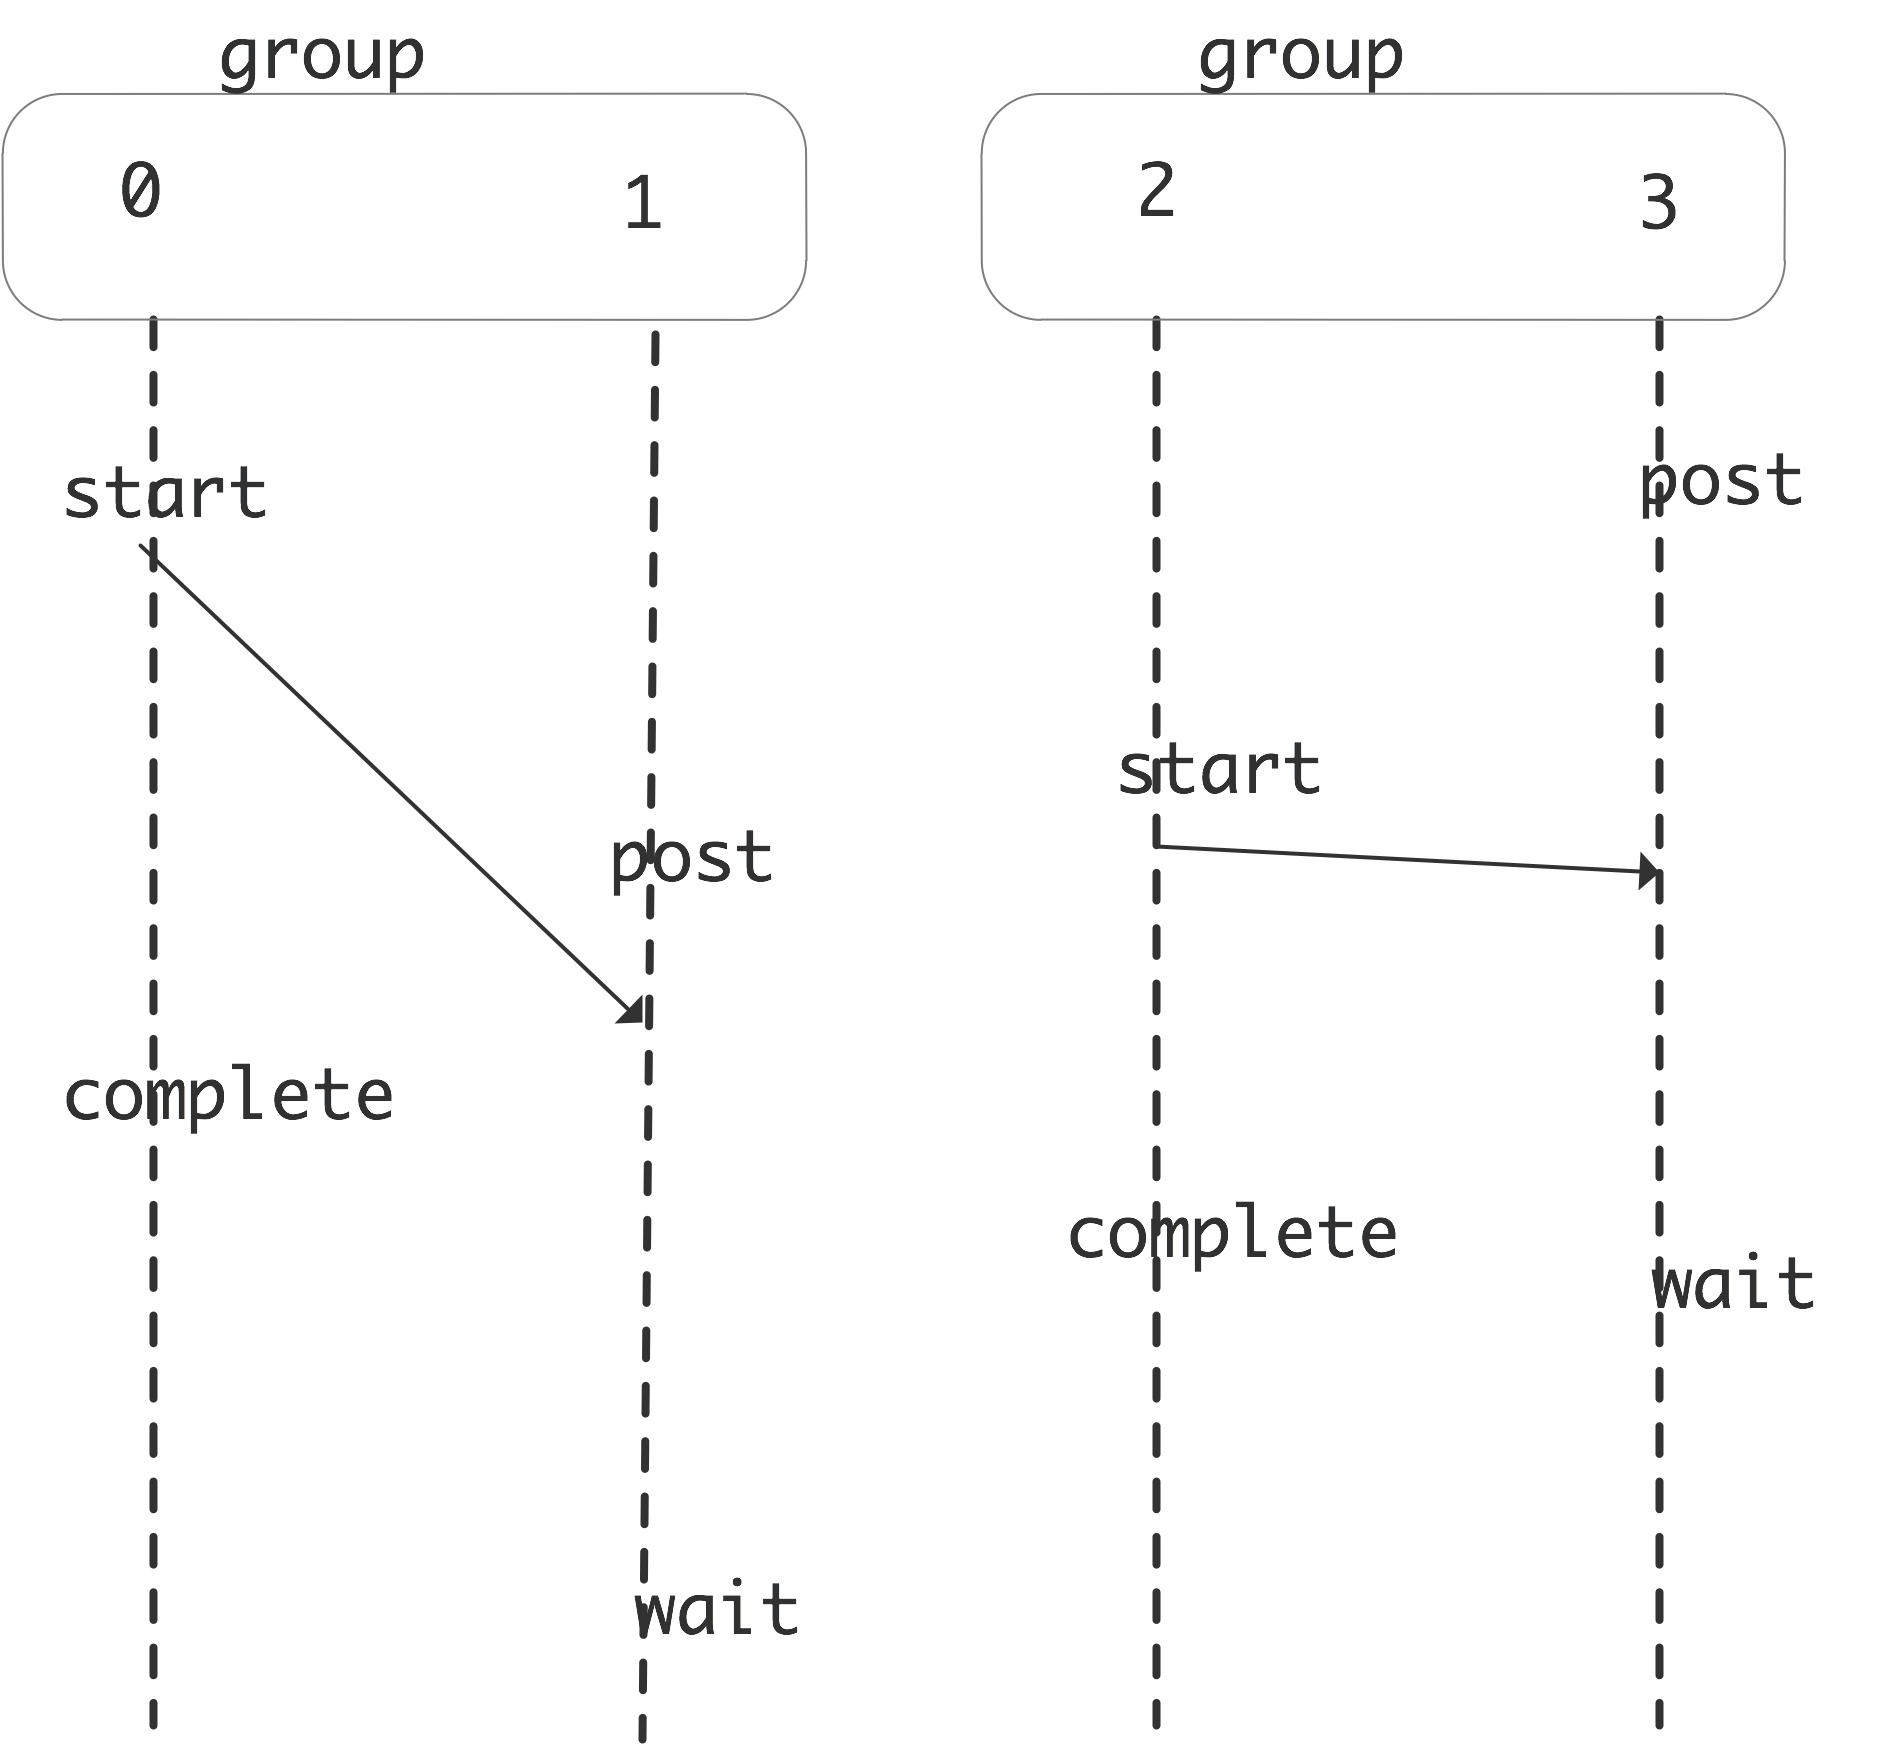
\includegraphics[scale=.1]{postwait}
  \caption{Window locking calls in fine-grained active target synchronization}
  \label{fig:postwait}
\end{figure}

You start and complete an \indextermsub{exposure}{epoch} with%
\indexmpi{MPI_Win_post}\indexmpi{MPI_Win_wait}:
\begin{verbatim}
int MPI_Win_post(MPI_Group group, int assert, MPI_Win win)
int MPI_Win_wait(MPI_Win win)
\end{verbatim}
In other words, this turns your window into the \indexterm{target} for a remote access.

You start and complete an \indextermsub{access}{epoch} with%
\indexmpi{MPI_Win_start}\indexmpi{MPI_Win_complete}:
\begin{verbatim}
int MPI_Win_start(MPI_Group group, int assert, MPI_Win win)
int MPI_Win_complete(MPI_Win win)
\end{verbatim}
In other words, these calls border the access to a remote window, with the current processor
being the \indexterm{origin} of the remote access.

In the following snippet a single processor puts data on one
other. Note that they both have their own definition of the group, and
that the receiving process only does the post and wait calls.
\verbatimsnippet{postwaittwo}

\Level 1 {Passive target synchronization}
\commandreflabel{passive-sync}

\indexmpi{MPI_Win_lock}\indexmpi{MPI_Win_unlock}
\begin{verbatim}
MPI_Win_lock (int locktype, int rank, int assert, MPI_Win win)
MPI_Win_unlock (int rank, MPI_Win win)
\end{verbatim}

The \indexmpi{MPI_Fetch_and_op} call atomically retrieves an item from the window
indicated, and replaces the item on the target by doing an accumulate on it
with the data on the origin.
%
\mpiRoutineRef{MPI_Fetch_and_op}

\Level 0 {Collectives}

\Level 1 {MPI Operators}

The following is the list of predefined \indexmpidef{MPI_OP} values.

\begingroup \tt\catcode`\_=12\relax
\begin{tabular}{ll}
  MPI_MAX&maximum\\
  MPI_MIN&minimum\\
  MPI_SUM&sum\\
  MPI_PROD&product\\
  MPI_LAND&logical and\\
  MPI_BAND&bitwise and\\
  MPI_LOR&logical or\\
  MPI_BOR&bitwise or\\
  MPI_LXOR&logical xor\\
  MPI_BXOR&bitwise xor\\
  MPI_MAXLOC&max value and location\\
  MPI_MINLOC&min value and location\\
\end{tabular}
\endgroup
All except the last two operate on MPI datatypes;
the last two operate on a value/index pair.

\Level 1 {`All'-type collectives}
\commandreflabel{allreduce}

The following collectives construct a result on all processes:
%
\mpiRoutineRef{MPI_Allgather}
%
\mpiRoutineRef{MPI_Allreduce}
%
\begin{pythonnote}
  The receive buffer has to be of the same size as the send buffer.
\end{pythonnote}

Each processor has a contribution in their send buffer; the global result
is returned in each processor's receive buffer.
\verbatimsnippet{allreduce}

If a large amount of data is being communicated, it may be wasteful to 
have both a (large) send and receive buffer.
This problem can be circumvented by using \indexmpishow{MPI_IN_PLACE}
as the specification of the send buffer. The send data is then
assumed to be in the receive buffer. After the reduction it is, of course,
overwritten.
\verbatimsnippet{allreduceinplace}

\Level 0 {Communicators}

\Level 1 {Communicator duplication}
\commandreflabel{comm-dup}

In section~\ref{sec:mpi-semantics} it was explained that MPI messages are 
non-overtaking. This may lead to confusing situations, witness the following snippet:

\verbatimsnippet{wrongcatchmain}

This models a main program that does a simple message exchange, and it
makes two calls to library routines. Unbeknown to the user, the
library also issues send and receive calls, and they turn out to
interfere:

\verbatimsnippet{wrongcatchlib}

Here
\begin{itemize}
\item The main program does a send,
\item the library call \n{function_start} does a send and a receive;
  because the receive can match either send, it is paired with the
  first one;
\item the main program does a receive, which will be paired with the send of the 
  library call;
\item both the main program and the library do a wait call, and in
  both cases all requests are succesfully fulfilled, just not the way
  you intended.
\end{itemize}

The solution is to give the library a separate communicator with
\indexmpishow{MPI_Comm_dup}.
%
\mpiRoutineRef{MPI_Comm_dup}
%
Newly created communicators should be
released again with \indexmpishow{MPI_Comm_free}.

\verbatimsnippet{rightcatchmain}

\Level 1 {Splitting communicators}
\commandreflabel{comm-split}

The command \indexmpishow{MPI_Comm_split} takes a communicator, and
divides it into a number of disjoint communicators. It does this by
assigning processes to the same subcommunicator if they have the same
user-specified `colour' value.
%
\mpiRoutineRef{MPI_Comm_split}
%
The ranking of processes in the new communicator is determined by a `key' value.
Most of the time, there is no reason to use a relative ranking that is different from
the global ranking, so the \n{MPI_Comm_rank} value of the global communicator
is a good choice.
\verbatimsnippet{commsplitrowcol}

There are some predefined colours, named `types', to use in communicator splitting.
The routine \indexmpishow{MPI_Comm_split_type} looks very much like \n{MPI_Comm_split}:
%
\mpiRoutineRef{MPI_Comm_split_type}
%
but the \n{split_type} parameters has to be from the following (short) list:
\begin{itemize}
\item \indexmpishow{MPI_COMM_TYPE_SHARED}: split the communicator into subcommunicators
  of processes sharing a memory area.
\end{itemize}

\Level 1 {Process topologies}
\commandreflabel{topology}

\Level 2 {Cartesian grid topology}
\commandreflabel{cartesian}

The cartesian topology is specified by giving
\indexmpishow{MPI_Cart_create} the sizes of the processor grid along
each axis, and whether the grid is periodic along that axis.
\begin{verbatim}
int MPI_Cart_create(
  MPI_Comm comm_old, int ndims, int *dims, int *periods, 
  int reorder, MPI_Comm *comm_cart)
\end{verbatim}
Each point in this new communicator has a coordinate and a rank.  They
can be queried with \indexmpishow{MPI_Cart_coord} and
\indexmpishow{MPI_Cart_rank} respectively.
\begin{verbatim}
int MPI_Cart_coords(
  MPI_Comm comm, int rank, int maxdims,
  int *coords);
int MPI_Cart_rank(
  MPI_Comm comm, init *coords, 
  int *rank);
\end{verbatim}
Note that these routines can give the coordinates for any rank,
not just for the current process.
%
\verbatimsnippet{cart}

The \n{reorder} parameter to \n{MPI_Cart_create}
indicates whether processes can have a rank
in the new communicator that is different from in the old one.

Strangely enough you can only shift in one direction, you can not
specify a shift vector.
\begin{verbatim}
int MPI_Cart_shift(MPI_Comm comm, int direction, int displ, int *source, 
                  int *dest)
\end{verbatim}
If you specify a processor outside the grid
the result is \indexmpishow{MPI_PROC_NULL}.

\Level 0 {Leftover topics}

\Level 1 {32-bit size issues}

The \n{size} parameter in MPI routines is defined as an \n{int},
meaning that it is limited to 32-bit quantities.  There are ways
around this, such as sending a number of
\indexmpishow{MPI_Type_contiguous} blocks that add up to more than~$2^{31}$.

\Level 1 {Fortran issues}
\commandreflabel{mpi-fortran}
\index{MPI!Fortran issues|(}

\Level 2 {Data types}

The equivalent of \indexmpishowsub{MPI_Aint}{in Fortran} is
\begin{verbatim}
integer(kind=MPI_ADDRESS_KIND) :: winsize
\end{verbatim}

\Level 2 {Type issues}

Fortran90 is a strongly typed language, so it is not possible to pass
argument by reference to their address, as C/C++ do with the \n{void*}
type for send and receive buffers. In Fortran this is solved by having
separate routines for each datatype, and providing an \n{Interface} block
in the MPI module. If you manage to request a version that does not exist,
the compiler will display a message like
\begin{verbatim}
There is no matching specific 
subroutine for this generic subroutine call [MPI_Send]
\end{verbatim}

\Level 2 {Byte calculations}
\label{sec:f-sizeof}

Fortran lacks a \n{sizeof} operator to query the sizes of datatypes.
Since sometimes exact byte counts are necessary,
for instance in one-sided communication,
Fortran can use the \indexmpishow{MPI_Sizeof} routine,
for instance for \indexmpishow{MPI_Win_create}:
\begin{verbatim}
call MPI_Sizeof(windowdata,window_element_size,ierr)
window_size = window_element_size*500
call MPI_Win_create( windowdata,window_size,window_element_size,... );
\end{verbatim}

\index{MPI!Fortran issues|)}

\Level 1 {Python issues}
\label{sec:python-stuff}
\index{MPI!Python issues|(}

\Level 2 {Byte calculations}

The \indexmpishow{MPI_Win_create} routine needs a displacement in
bytes. Here is a good way for finding the size of \indexterm{numpy} datatypes:
\begin{verbatim}
numpy.dtype('i').itemsize
\end{verbatim}

\Level 2 {Arrays of objects}

Objects of type \n{MPI.Status} or \n{MPI.Request} often need to be created
in an array, for instance when looping through a number of \n{Isend} calls.
In that case the following idiom may come in handy:
\begin{verbatim}
requests = [ None ] * nprocs
for p in range(nprocs):
  requests[p] = comm.Irecv( ... )
\end{verbatim}

\index{MPI!Python issues|)}

\Level 1 {Cancelling messages}

In section~\ref{sec:mpi-source} we showed a master-worker example where the 
master accepts in arbitrary order the messages from the workers.
Here we will show a slightly
more complicated example, where only the result of the first task to
complete is needed. Thus, we issue an \n{MPI_Recv}
with \indexmpishow{MPI_ANY_SOURCE} as source.  When a result comes, we
broadcast its source to all processes.  All the other workers then use
this information to cancel their message with
an \indexmpishow{MPI_Cancel} operation.

\verbatimsnippet{cancel}

\Level 1 {Constants}

MPI constants such as \n{MPI_COMM_WORLD} or \n{MPI_INT} are not
necessarily statitally defined, such as by a \n{#define} statement:
the best you can say is that they have a value after
\indexmpishow{MPI_Init} or \indexmpishow{MPI_Init_thread}.
That means you can not transfer a compiled MPI file between
platforms, or even between compilers on one platform.
However, a working MPI source on one MPI implementation
will also work on another.

\Level 0 {Error handling}
\commandreflabel{mpi:error}

MPI operators (\indexmpishow{MPI_Op}) do not return an error code. In case of
an error they call \n{MPI_Abort}; if \indexmpishow{MPI_ERRORS_RETURN}
is the error handler, errors may be silently ignore.

\Level 0 {Context information}
\label{sec:context}

\Level 1 {Processor name}

You can query the \indexterm{hostname} of a processor.
This name need not be unique between different processor ranks.
%
\mpiRoutineRef{MPI_Get_processor_name}
%
Note that you have to pass in the character storage:
the character array must be at least \indexmpishow{MPI_MAX_PROCESSOR_NAME} characters long.
The actual length of the name is returned in the \n{resultlen} parameter.

In C and C++,
\begin{verbatim}
  #define MPI_VERSION 2
  #define MPI_SUBVERSION 2
\end{verbatim}
in Fortran,
\begin{verbatim}
  INTEGER MPI_VERSION, MPI_SUBVERSION
  PARAMETER (MPI_VERSION = 2)
  PARAMETER (MPI_SUBVERSION = 2)
\end{verbatim}
For runtime determination,
\begin{verbatim}
  MPI_GET_VERSION( version, subversion )
  OUT version version number (integer)
  OUT subversion subversion number (integer)

  int MPI_Get_version(int *version, int *subversion)
  MPI_GET_VERSION(VERSION, SUBVERSION, IERROR)
  INTEGER VERSION, SUBVERSION, IERROR
\end{verbatim}

\Level 1 {Attributes}

\mpiRoutineRef{MPI_Attr_get}

Attributes are:
\begin{itemize}
\item \indexmpishow{MPI_UNIVERSE_SIZE}: the total number of processes
  that can be created. This can be more than the size of
  \n{MPI_COMM_WORLD} if the host list is larger than the number of
  initially started processes. See section~\ref{sec:mpi-dynamic}.
\item \indexmpishow{MPI_APPNUM}: if MPI is used in \ac{MPMD} mode, or
  if \indexmpishow{MPI_Comm_spawn_multiple} is used, this attribute
  reports the how-manieth program we are in.
\end{itemize}

\Level 0 {Timing}
\commandreflabel{mpi-timing}

MPI has a \indexterm{wall clock} timer: \indexmpishow{MPI_Wtime}
\begin{verbatim}
// C
double MPI_Wtime(void);
! F
DOUBLE PRECISION MPI_WTIME()
\end{verbatim}
which gives the number of seconds from a certain point in the past.
(Note the absence of the error parameter in the fortran call.)
\verbatimsnippet{pingpong}

The timer has a resolution of \indexmpishow{MPI_Wtick}:
\begin{verbatim}
double MPI_Wtick(void);
\end{verbatim}

Timing in parallel is a tricky issue. For instance, most clusters do
not have a central clock, so you can not relate start and stop times
on one process to those on another. You can test for a global clock as
follows\indexmpi{MPI_WTIME_IS_GLOBAL}:
\begin{verbatim}
int *v,flag;
MPI_Attr_get( comm, MPI_WTIME_IS_GLOBAL, &v, &flag );
if (mytid==0) printf(``Time synchronized? %d->%d\n'',flag,*v);
\end{verbatim}
%\indexmpi{MPI_Wtime} can be either a function or a macro.

%\Level 1 {Profiling}
%\commandreflabel{profile}

\Level 0 {Multi-threading}
\commandreflabel{mpi-thread}

Hybrid MPI/threaded codes need to replace \indexmpishow{MPI_Init}
by \n{MPI_Init_thread}:
%
\mpiRoutineRef{MPI_Init_thread}
%
With the \n{required} parameter the user requests a certain level of support,
and MPI reports the actual capabilities in the \n{provided} parameter.

The following constants are defined:
\begin{itemize}
\item \indexmpishow{MPI_THREAD_SINGLE}: each MPI process can only have
  a single thread.
\item \indexmpishow{MPI_THREAD_FUNNELED}: an MPI process can be
  multithreaded, but all MPI calls need to be done from a single
  thread.
\item \indexmpishow{MPI_THREAD_SERIALIZED}: a processes can sustain
  multiple threads that make MPI calls, but these threads can not be
  simultaneous: they need to be for instance in an OpenMP
  \indexterm{critical section}.
\item \indexmpishow{MPI_THREAD_MULTIPLE}: processes can be fully
  generally multi-threaded.
\end{itemize}
These values are monotonically increasing.

After the initialization call, you can query the support level
with \n{MPI_Query_thread}:
%
\mpiRoutineRef{MPI_Query_thread}

In case more than one thread performs communication, the following routine
can determine whether a thread is the main thread:
%
\mpiRoutineRef{MPI_Is_thread_main}
